\documentclass[fleqn, a4paper, 11pt, oneside]{amsart}
%\usepackage[top = 2cm, bottom = 1cm, left = 1cm, right = 1cm]{geometry}
\usepackage{exsheets, tasks}
\usepackage{amsmath, amssymb, amsthm} %standard AMS packages
\usepackage{marginnote} %marginnotes
\usepackage{gensymb} %miscellaneous symbols
\usepackage{commath} %differential symbols
\usepackage{xcolor} %colours
\usepackage{cancel} %cancelling terms
\usepackage{siunitx} %formatting units
\usepackage{tikz, pgfplots} %diagrams
\usetikzlibrary{calc, hobby, patterns, intersections}
\usepackage{graphicx} %inserting graphics
\usepackage{hyperref} %hyperlinks
\usepackage{datetime} %date and time
\usepackage{ulem} %underline for \emph{}
\usepackage{xfrac} %inline fractions
\usepackage{enumerate,enumitem} %numbered lists
\usepackage{float} %inserting floats
\usepackage{circuitikz}[american voltages, american currents] %circuit diagrams

\newcommand\numberthis{\addtocounter{equation}{1}\tag{\theequation}} %adds numbers to specific equations in non-numbered list of equations

\newcommand{\AxisRotator}[1][rotate=0]{
	\tikz [x=0.25cm,y=0.60cm,line width=.2ex,-stealth,#1] \draw (0,0) arc (-150:150:1 and 1);%
} %rotation symbols on axes

\theoremstyle{definition}
\newtheorem{example}{Example}
\newtheorem{definition}{Definition}

\theoremstyle{theorem}
\newtheorem{theorem}{Theorem}

\newcommand{\curl}{\mathrm{curl\,}}

\makeatletter
\@addtoreset{section}{part} %resets section numbers in new part
\makeatother

\renewcommand{\thesubsection}{(\arabic{subsection})}
\renewcommand{\thesection}{(\arabic{section})}

%section headings on left
\makeatletter
\def\specialsection{\@startsection{section}{1}%
	\z@{\linespacing\@plus\linespacing}{.5\linespacing}%
	%  {\normalfont\centering}}% DELETED
	{\normalfont}}% NEW
\def\section{\@startsection{section}{1}%
	\z@{.7\linespacing\@plus\linespacing}{.5\linespacing}%
	%  {\normalfont\scshape\centering}}% DELETED
	{\normalfont\scshape}}% NEW
\makeatother

%forces newline after subsection
\makeatletter
\def\subsection{\@startsection{subsection}{3}%
	\z@{.5\linespacing\@plus.7\linespacing}{.1\linespacing}%
	{\normalfont\itshape}}
\makeatother

\settasks{counter-format = tsk[1].}

\SetupExSheets{solution/print = true}

%opening
\title{Physics 2 : Assignment 8}
\author
{
	Aakash Jog\\
	ID : 989323563
}
\date{\formatdate{20}{5}{2015}}

\begin{document}

\maketitle
%\setlength{\mathindent}{0pt}

\begin{question}
	\begin{enumerate}
		\item
			Find the magnetic field at the center of a square loop, which carries a steady current $I$.
			Let $R$ be the distance from the center to a side.
		\item
			Find the field at the center of a regular $n$-sided polygon, carrying steady current $I$.
			Again, let $R$ be the distance from the center to a side.
		\item
			Check that your formula reduces to the field at the center of a circular loop, for the limit $n \to \infty$.
	\end{enumerate}
\end{question}

\begin{solution}
	\begin{enumerate}[leftmargin = *]
		\item
			Let the angle between the line joining a point, at a perpendicular distance $R$ from the centre of a straight wire of length $L$, and the end of the wire; and the wire, be $\theta_0$.\\
			The magnetic field at the point due to the wire is
			\begin{align*}
				\overrightarrow{B_{\textnormal{line}}} &= \frac{\mu_0}{4 \pi} \int \frac{\overrightarrow{I \dif l} \times \hat{r}}{r^2}\\
				\therefore B &= \frac{\mu_0 I}{4 \pi R} \cdot 2 \sin \theta
				&= \frac{\mu_0 I \sin \theta}{2 \pi R}
			\end{align*}
			The magnetic field due to each of the sides of the loop is pointing in the same direction, perpendicular to the plane of the loop, as determined by the right hand thumb rule.
			Therefore, the magnitude of the net field at the centre is the sum of the magnitudes of the magnetic fields at the centre due to each of the sides.\\
			Therefore,
			\begin{align*}
				B &= 4 \left( \frac{\mu_0 I \sin \theta}{2 \pi R} \right)\\
				&= 4 \left( \frac{\mu_0 I \sin \frac{\pi}{4}}{2 \pi R} \right)\\
				&= 4 \left( \frac{\mu_0 I}{2 \sqrt{2} \pi R} \right)\\
				&= \frac{\sqrt{2} \mu_0 I}{\pi R}
			\end{align*}
		\item
			The angle subtended by the side of a regular $n$-sided polygon at the centre is $\frac{2 \pi}{n}$.\\
			Therefore, $\theta = \frac{\frac{2 \pi}{n}}{2} = \frac{\pi}{n}$.\\
			Therefore,
			\begin{align*}
				B &= n \left( \frac{\mu_0 I \sin \theta}{2 \pi R} \right)\\
				&= n \left( \frac{\mu_0 I \sin \frac{\pi}{n}}{2 \pi R} \right)\\
				&= \frac{n \mu_0 I \sin \frac{\pi}{n}}{2 \pi R}
			\end{align*}
		\item
			As $n \to \infty$, $\frac{\pi}{n} \to 0$.\\
			Therefore, $\sin \frac{\pi}{n} = \frac{\pi}{n}$.\\
			Therefore,
			\begin{align*}
				B &= \frac{n \mu_0 I \frac{\pi}{n}}{2 \pi R}\\
				&= \frac{\mu_0 I}{2 \pi R}
			\end{align*}
	\end{enumerate}
\end{solution}

\begin{question}
	Find the magnetic field at point $P$ for each of the steady current configurations shown.
	\begin{enumerate}[leftmargin = *]
		\item
			\begin{figure}[H]
				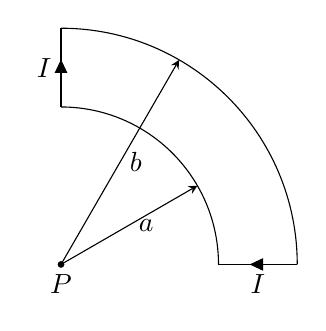
\begin{tikzpicture}
					\def\a{2};
					\def\b{3};
		
					\draw (\a,0) arc (0:90:\a);
					\draw (\b,0) arc (0:90:\b);
					\draw (\b,0) to [short, i = $I$] (\a,0);
					\draw (0,\a) to [short, i = $I$] (0,\b);
		
					\begin{scope}[-stealth]
						\draw (0,0) -- (30:\a) node [midway, right] {$a$};
						\draw (0,0) -- (60:\b) node [midway, right] {$b$};
					\end{scope}

					\filldraw (0,0) circle (1pt) node [below] {$P$};
				\end{tikzpicture}
			\end{figure}
		\item
			\begin{figure}[H]
				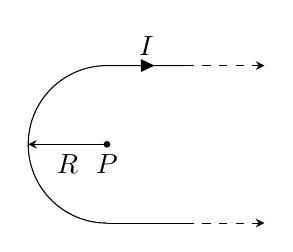
\begin{tikzpicture}
					\def\R{1};
					\def\L{1};
	
					\draw (0,\R) arc (90:270:\R);
	
					\draw (0,\R) to[short, i = $I$] ++(0:\L);
					\draw[dashed, -stealth] (\L,\R) -- ++(0:\L);
	
					\draw (0,-\R) -- ++(0:\L);
					\draw[dashed, -stealth] (\L,-\R) -- ++(0:\L);

					\begin{scope}[-stealth]
						\draw (0,0) -- (-\R,0) node [midway, below] {$R$};
					\end{scope}

					\filldraw (0,0) circle (1pt) node [below] {$P$};
				\end{tikzpicture}
			\end{figure}
	\end{enumerate}
\end{question}

\begin{solution}
	\begin{enumerate}[leftmargin = *]
		\item
			As the straight wires are carrying current in the direction of $P$, the magnetic field due to them is zero.
			Therefore, the net field is due to the arcs only.\\
			The field due to the inner arc is pointing outwards, and the field due to the outer arc is pointing inwards.\\
			As the field due to the inner arc is stronger in magnitude, the net field will be directed outwards.\\
			Therefore,
			\begin{align*}
				B &= \frac{1}{4} \frac{\mu_0 I}{2 a} - \frac{1}{4} \frac{\mu_0 I}{2 b}\\
				&= \frac{\mu_0 I}{8} \left( \frac{1}{a} - \frac{1}{b} \right)
			\end{align*}
		\item
			\begin{align*}
				B_{\textnormal{end of infinite line}} &= \frac{\mu_0 I}{4 \pi R} (\sin \frac{\pi}{2} - \sin 0)
			\end{align*}
			Therefore,
			\begin{align*}
				B &= \frac{1}{2} \frac{\mu_0 I}{2 R} + 2 \left( \frac{\mu_0 I}{4 \pi R} \right)\\
				&= \frac{\mu_0 I}{4 R} + \frac{\mu_0 I}{2 \pi R}
			\end{align*}
			By the right hand thumb rule, $\overrightarrow{B}$ is directed inwards.
	\end{enumerate}
\end{solution}

\begin{question}
	A particle of charge $q$ enters a region of uniform magnetic field $B⃗$ (pointing into the page).
	The field deflects the particle a distance $d$ above the original line of flight, as shown.
	\begin{figure}[H]
		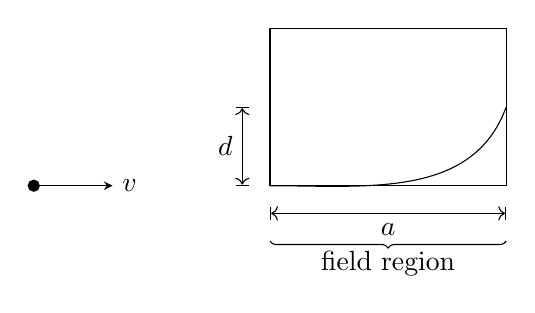
\begin{tikzpicture}
			\def\a{3};
			\def\d{1};
			\def\F{1};

			\begin{scope}
				\draw (0,0) rectangle (\a,\d + 1);
			\end{scope}

			\begin{scope}[|<->|]
				\draw[yshift = -10] (0,0) -- (\a,0) node[midway, below] {$a$};
				\draw[xshift = -10] (0,0) -- (0,\d) node[midway, left] {$d$};
			\end{scope}

			\draw[yshift = -20, decorate, decoration = {mirror, brace}] (0,0) -- (\a,0) node[midway, below] {field region};

			\begin{scope}
				\filldraw (-\a,0) circle (2pt);
				\draw[-stealth] (-\a,0) -- ++(0:\F) node [right] {$v$};
			\end{scope}

			\begin{scope}
				\draw (0,0) to [out = 0, in = 250] (\a,\d);
			\end{scope}
		\end{tikzpicture}
	\end{figure}
	Is the charge positive or negative?
	In terms of $a$, $\dif \overrightarrow{B}$ and $q$, find the momentum of the particle.
\end{question}

\begin{solution}
	\begin{figure}[H]
		\begin{tikzpicture}
			\begin{scope}[-stealth]
				\draw (0,0) -- (1,0) node [right] {$v$};
				\draw (0,0) -- (0,1) node [above] {$F$};

				\node at (0,0) {$\otimes$};
				\node at (-0.5,0) {$B$};
			\end{scope}
		\end{tikzpicture}
	\end{figure}
	The directions of $\overrightarrow{v}$, $\overrightarrow{B}$ and $\overrightarrow{F}$ are as shown.\\
	Therefore, as $\hat{v} \times \hat{B} = \hat{F}$, $q$ must be positive.
	\begin{align*}
		R^2 &= (R - d)^2 + a^2\\
			&= R^2 - 2 R d + d^2 + a^2\\
		\therefore R &= \frac{a^2 + d^2}{2 d}
	\end{align*}
	Therefore,
	\begin{align*}
		\frac{m v^2}{R} &= q v B\\
		\therefore \frac{p v}{R} &= q v B\\
		\therefore p &= R q B\\
		&= \frac{a^2 + d^2}{2 d} q B
	\end{align*}
\end{solution}

\begin{question}
	A capacitor $C$ has been charged $U_0$ to potential $V_0$.
	At time $t = 0$ it is connected to a resistor $R$, and begins to discharge.
	\begin{figure}[H]
		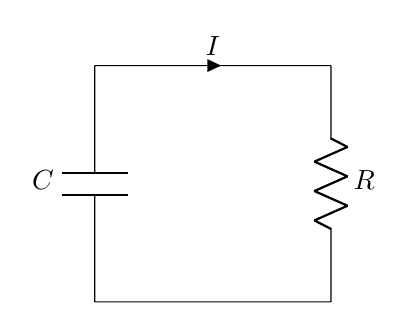
\begin{tikzpicture}
			\draw
				(0,0) to [C = $C$] (0,3)
				(0,3) to [short, i = $I$] (3,3)
				(3,3) to [R = $R$] (3,0)
				(3,0) to (0,0);
		\end{tikzpicture}
	\end{figure}
	\begin{enumerate}
		\item Determine the charge on the capacitor and the current through the resistor as a function of time $Q(t)$ and $I(t)$.
		\item Show that the heat delivered to the resistor is equal to the energy originally stored in the capacitor.
	\end{enumerate}
	Now imagine charging up the capacitor, by connecting it (and the resistor) to a battery of fixed voltage $V_0$, at time $t = 0$.
	\begin{figure}[H]
		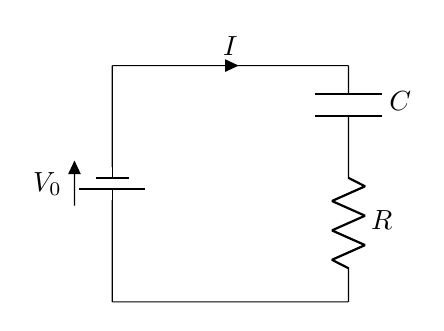
\begin{tikzpicture}
			\draw
				(0,0) to [battery1 = $V_0$] (0,3)
				(0,3) to [short, i = $I$] (3,3)
				(3,3) to [C = $C$] (3,2)
				(3,2) to [R = $R$] (3,0)
				(3,0) to (0,0);
		\end{tikzpicture}
	\end{figure}
	\begin{enumerate}[resume]
		\item Again determine $Q(t)$ and $I(t)$.
		\item
			Find the total energy output of the battery ($V_0 I \dif t$).
			Determine the heat delivered to the resistor.
			What is the final energy stored in the capacitor?
			What fraction of the work done by the battery shows up as energy in the capacitor? (notice that the answer is independent of $R$!)
	\end{enumerate}
\end{question}

\begin{solution}
	\begin{enumerate}[leftmargin = *]
		\item
			By KVL,
			\begin{align*}
				V_R + V_C &= 0
			\end{align*}
			Therefore,
			\begin{align*}
				\frac{Q}{C} &= -I R\\
				\therefore \frac{Q}{C} &= \dod{Q}{t} R\\
				\therefore Q' + \frac{1}{R C} Q - \frac{1}{R} &= 0
			\end{align*}
			Therefore, solving and substituting $Q(t = 0) = C V_0$,
			\begin{align*}
				Q &= C V_0 e^{-\frac{t}{R C}}
			\end{align*}
			Therefore,
			\begin{align*}
				I &= C V_0 \frac{1}{R C} e^{-\frac{t}{R C}}\\
				&= \frac{V_0}{R} e^{-\frac{t}{R C}}
			\end{align*}
		\item
			\begin{align*}
				E_R &= \int\limits_{0}^{\infty} I^2 R \dif t\\
				&= \int\limits_{0}^{\infty} \left( \frac{V_0}{R} e^{-\frac{t}{R C}} \right)^2 R \dif t\\
				&= \int\limits_{0}^{\infty} \frac{{V_0}^2}{R} e^{-\frac{2 t}{R C}} \dif t\\
				&= \frac{{V_0}^2}{R} \left. \left( -\frac{R C}{2} e^{-\frac{2 t}{R C}} \right) \right|_{0}^{\infty}\\
				&= \frac{1}{2} C {V_0}^2
			\end{align*}
		\item
			By KVL,
			\begin{align*}
				V_0 &= V_R + V_C
			\end{align*}
			Therefore,
			\begin{align*}
				V_0 &= \frac{Q}{C} + I R\\
				&= \frac{Q}{C} + Q' R\\
				\therefore Q' + \frac{1}{R C} Q - \frac{V_0}{R} &= 0
			\end{align*}
			Therefore, solving and substituting $Q(t = 0) = 0$,
			\begin{align*}
				Q &= C V_0 \left( 1 - e^{-\frac{t}{R C}} \right)
			\end{align*}
			Therefore,
			\begin{align*}
				I &= C V_0 \left( \frac{1}{R C} e^{-\frac{t}{R C}} \right)\\
				&= \frac{V_0}{R} e^{-\frac{t}{R C}}
			\end{align*}
		\item
			\begin{align*}
				E_{\textnormal{battery}} &= \int\limits_{0}^{\infty} V_0 I \dif t\\
				&= \int\limits_{0}^{\infty} V_0 \frac{V_0}{R} e^{-\frac{t}{R C}} \dif t\\
				&= \frac{{V_0}^2}{R} \int\limits_{0}^{\infty} e^{-\frac{t}{R C}}\\
				&= \frac{{V_0}^2}{R} \left. \left( -R C e^{-\frac{t}{R C}} \right) \right|_{0}^{\infty}\\
				&= \frac{{V_0}^2}{R} R C\\
				&= C {V_0}^2
			\end{align*}
			Therefore, the net energy supplied by the battery is $C {V_0}^2$.
			Out of these, $\frac{1}{2} C {V_0}^2$ is stored on the capacitor and the remaining is dissipated at the resistor.\\
			Therefore, half the energy goes to the capacitor.
	\end{enumerate}
\end{solution}

\end{document}
